\section{Google Fusion Table JavaScript Library (GftLib)}
\label{gftlib-js}
Die Google Fusion Table JavaScript Library (GftLib) ist eine von uns entwickelte JavaScript Bibliothek, welche die Kommunikation mit dem Google Fusion Table SQL \gls{API} (siehe Abschnitt \ref{sql-api}) vereinfacht. Sie hilft dabei, SQL-Abfragen zu erstellen und diese per \gls{AJAX} an das \gls{API} zu senden. Zudem kümmert sich die Library um die Authentifizierung via \gls{OAuth}, so dass auch schreibende Zugriffe oder Zugriffe auf private Tabellen möglich sind.

Die Bibliothek hat Abhängigkeiten zu jQuery\footnote{\url{http://jquery.com/}} (für einige Hilfsfunktionen) sowie dem Google \gls{API} JavaScript Client\footnote{\url{http://code.google.com/p/google-api-javascript-client/}} (für die Authentifizierung und das Abschicken der Requests).

Die Bibliothek besteht aus zwei Klassen (GftLib und SqlBuilder). Die GftLib ist das \gls{API} zum Client und steuert dementsprechend die Requests und die Authentifizierung. Der SqlBuilder ist eine Hilfsklasse, welche es erlaubt, auf einfach Art und Weise SQL-Befehle zu generieren.

\subsection{Verwendung}
Im Code-Beispiel \ref{gftlib-example} sieht man die GftLib und den SqlBuilder im Einsatz. Zuerst werden alle benötigten Werte initialisiert (Zeilen 1-3), dann wird die Ausgabefunktion \inlinecode{printer} definiert, welche später als Callback-Funktion dient für den Request. Das heisst, dass die Funktion aufgerufen wird, sobald die Antwort der Abfrage zurückkommt. 

Mit der Funktion \inlinecode{convertToObject()} wird die Antwort von Google Fusion Tables in eine für den Benutzer besser verständliche Form umgewandelt. Das Resultat der Fusion Tables kommt in Form eines zweidimensionalen Arrays zurück, welches für jeden Datensatz alle abgefragten Felder enthält. Die Funktion erstellt jeweils pro Datensatz ein Objekt, welches die angefragten Felder als Properties hat. So kann man mit deren Namen auf ihre Werte zugreifen (z.B. \inlinecode{places[i].name} oder \inlinecode{places[i].population}).

In diesem Beispiel wird das SQL Query direkt in der Funktion \inlinecode{execSelect()} erzeugt, welche dazu den SqlBuilder verwendet.

\lstset{language=JavaScript}
\begin{lstlisting}[caption=Verwendung der GftLib, label=gftlib-example]
var tableId = '1LWXSMsZINyfjAKGqeS-822wi4WmlaGmmvh20Ujw';
var gft = new GftLib();
var resultList = document.getElementById("result");

var printer = function(data) {
	var places = gft.convertToObject(data);

	for (var i = 0; i < places.length; i++) {
		var listElem = document.createElement('li');
		listElem.innerHTML = 'Place: ' + places[i].name + ' / Population: ' + places[i].population;
		resultList.appendChild(listElem);
	}
}

gft.execSelect(printer, {table:tableId, fields:['name', 'population']});
\end{lstlisting}

\subsection{Abhängigkeiten}
\begin{table}[H]
\centering
\begin{tabular}{|p{0.3\threecelltabwidth}|p{0.2\threecelltabwidth}|p{0.5\threecelltabwidth}|}
\hline 
\textbf{Library} & \textbf{Version} & \textbf{Verwendung} \\ 
\hline 
jQuery & 1.7.1-min & Helper-Funktionen und \gls{AJAX}-Requests für den OAuthTokenService  \\ 
\hline 
Google \gls{API}s Client Library & ALPHA release & \gls{AJAX}-Requests an das Google \gls{API} und Authentifizierung \\ 
\hline 
\end{tabular} 
\caption{Abhängigkeiten der GftLib}
\end{table}

\subsection{Methoden}
\subsubsection{GftLib}
\begin{longtable}{|p{0.3\threecelltabwidth}|p{0.2\threecelltabwidth}|p{0.5\threecelltabwidth}|}
\hline 
\textbf{Methode} & \textbf{Beschreibung} & \textbf{Parameter} \\ 
\hline 
\inlinecode{execQuery( callback, query )} &  Führt eine SQL-Abfrage aus & 
\begin{itemize}[noitemsep, nosep, leftmargin=12pt, before*={\mbox{}\vspace{-\baselineskip}}, after*={\mbox{}\vspace{-\baselineskip}}]
\item \inlinecode{callback}: Callback-Methode, welche nach Beendigung der Methode aufgerufen wird. 
\item \inlinecode{query}: SQL-Query
\end{itemize} \\ 
\hline 
\inlinecode{execSql( callback, sql )} & Führt einen beliebigen SQL-Befehl aus & 
\begin{itemize}[noitemsep, nosep, leftmargin=12pt, before*={\mbox{}\vspace{-\baselineskip}}, after*={\mbox{}\vspace{-\baselineskip}}]
\item \inlinecode{callback}: Callback-Methode, welche nach Beendigung der Methode aufgerufen wird. 
\item \inlinecode{sql}: SQL-Befehl
\end{itemize} \\ 
\hline 
\inlinecode{execSelect( callback, options )} & Führt eine \inlinecode{SELECT}-Abfrage aus & 
\begin{itemize}[noitemsep, nosep, leftmargin=12pt, before*={\mbox{}\vspace{-\baselineskip}}, after*={\mbox{}\vspace{-\baselineskip}}]
\item \inlinecode{callback}: Callback-Methode, welche nach Beendigung der Methode aufgerufen wird.
\item \inlinecode{options}: Parameter-Objekt für \inlinecode{SqlBuilder.selectStmt()}
\end{itemize} \\ 
\hline
\inlinecode{execInsert( callback, options )} & Führt einen \inlinecode{INSERT}-Befehl aus & 
\begin{itemize}[noitemsep, nosep, leftmargin=12pt, before*={\mbox{}\vspace{-\baselineskip}}, after*={\mbox{}\vspace{-\baselineskip}}]
\item \inlinecode{callback}: Callback-Methode, welche nach Beendigung der Methode aufgerufen wird.
\item \inlinecode{options}: Parameter-Objekt für \inlinecode{SqlBuilder.insertStmt()}
\end{itemize} \\ 
\hline
\inlinecode{execUpdate( callback, options )} & Führt einen \inlinecode{UPDATE}-Befehl aus &
\begin{itemize}[noitemsep, nosep, leftmargin=12pt, before*={\mbox{}\vspace{-\baselineskip}}, after*={\mbox{}\vspace{-\baselineskip}}]
\item \inlinecode{callback}: Callback-Methode, welche nach Beendigung der Methode aufgerufen wird. 
\item \inlinecode{options}: Parameter-Objekt für \inlinecode{SqlBuilder.updateStmt()}
\end{itemize} \\ 
\hline 
\inlinecode{execDelete( callback, options )} & Führt einen \inlinecode{DELETE}-Befehl aus & 
\begin{itemize}[noitemsep, nosep, leftmargin=12pt, before*={\mbox{}\vspace{-\baselineskip}}, after*={\mbox{}\vspace{-\baselineskip}}]
\item \inlinecode{callback}: Callback-Methode, welche nach Beendigung der Methode aufgerufen wird.
\item \inlinecode{options}: Parameter-Objekt für \inlinecode{SqlBuilder.deleteStmt()} 
\end{itemize} \\ 
\hline 
\inlinecode{getTableDescription( callback, options )} & Führt eine \inlinecode{DESCRIBE}-Abfrage aus & 
\begin{itemize}[noitemsep, nosep, leftmargin=12pt, before*={\mbox{}\vspace{-\baselineskip}}, after*={\mbox{}\vspace{-\baselineskip}}]
\item \inlinecode{callback}: Callback-Methode, welche nach Beendigung der Methode aufgerufen wird. 
\item \inlinecode{options}: Parameter-Objekt für \inlinecode{SqlBuilder.describeStmt()}
\end{itemize} \\
\hline 
\inlinecode{createView( callback, options )} & Führt einen \inlinecode{CREATE VIEW}-Befehl aus & 
\begin{itemize}[noitemsep, nosep, leftmargin=12pt, before*={\mbox{}\vspace{-\baselineskip}}, after*={\mbox{}\vspace{-\baselineskip}}]
\item \inlinecode{callback}: Callback-Methode, welche nach Beendigung der Methode aufgerufen wird. 
\item \inlinecode{options}: Parameter-Objekt für \inlinecode{SqlBuilder.createViewStmt()} 
\end{itemize} \\ 
\hline 
\inlinecode{convertToObject( gftData )} & Konvertiert das Resultat einer Abfrage in sprechende Objekte & 
\begin{itemize}[noitemsep, nosep, leftmargin=12pt, before*={\mbox{}\vspace{-\baselineskip}}, after*={\mbox{}\vspace{-\baselineskip}}]
\item \inlinecode{gftData}: Antwort auf einen SQL Befehl von Google Fusion Tables
\end{itemize} \\ 
\hline 
\caption{Methoden der GftLib-Klasse}
\end{longtable} 

\subsubsection{SqlBuilder}
Die Methoden des SqlBuilders nehmen jeweils ein Parameter-Objekt\footnote{\url{http://www.refactoring.com/catalog/introduceParameterObject.html}} entgegen und erstellen daraus SQL-Befehle, welche dann als Input für die GftLib gebraucht werden können.

\begin{longtable}{|p{0.3\threecelltabwidth}|p{0.2\threecelltabwidth}|p{0.5\threecelltabwidth}|}
\hline 
\textbf{Methode} & \textbf{Beschreibung} & \textbf{Parameter} \\ 
\hline
\inlinecode{selectStmt( options )} & Generiert ein \inlinecode{SELECT} Statement & 
\inlinecode{options}: Parameter-Objekt mit folgenden Feldern:
\begin{itemize}[noitemsep]
\item \inlinecode{fields}: Array von Feldernamen (Default *)
\item \inlinecode{table}: ID der Tabelle oder View
\item \inlinecode{conditions}: Array von Bedingungen für die \inlinecode{WHERE}-Klausel 
\end{itemize}\\
\hline
\inlinecode{insertStmt( options )} & Generiert ein \inlinecode{INSERT} Statement & 
\inlinecode{options}: Parameter-Objekt mit folgenden Feldern:
\begin{itemize}[noitemsep]
\item \inlinecode{fields}: Array von Feldernamen
\item \inlinecode{table}: ID der Tabelle oder View
\item \inlinecode{values}: Array von Werten (in der gleichen Reihenfolge wie \inlinecode{fields})
\end{itemize}\\
\hline
\inlinecode{updateStmt( options )} & Generiert ein \inlinecode{UPDATE} Statement & 
\inlinecode{options}: Parameter-Objekt mit folgenden Feldern:
\begin{itemize}[noitemsep]
\item \inlinecode{fields}: Array von Feldernamen
\item \inlinecode{table}: ID der Tabelle oder View
\item \inlinecode{values}: Array von Werten (in der gleichen Reihenfolge wie \inlinecode{fields})
\item \inlinecode{conditions}: Array von Bedingungen für die \inlinecode{WHERE}-Klausel
\end{itemize}\\
\hline
\inlinecode{deleteStmt( options )} & Generiert ein \inlinecode{DELETE} Statement & 
\inlinecode{options}: Parameter-Objekt mit folgenden Feldern:
\begin{itemize}[noitemsep]
\item \inlinecode{table}: ID der Tabelle oder View
\item \inlinecode{conditions}: Array von Bedingungen für die \inlinecode{WHERE}-Klausel
\end{itemize}\\
\hline
\inlinecode{describeStmt( options )} & Generiert ein \inlinecode{DESCRIBE} Statement & 
\inlinecode{options}: Parameter-Objekt mit folgenden Feldern:
\begin{itemize}[noitemsep]
\item \inlinecode{table}: ID der Tabelle oder View
\end{itemize}\\
\hline
\inlinecode{createViewStmt( options )} & Generiert ein \inlinecode{CREATE VIEW} Statement & 
\inlinecode{options}: Parameter-Objekt mit folgenden Feldern:
\begin{itemize}[noitemsep]
\item \inlinecode{viewName}: Name der neuen View
\item \inlinecode{query}: Ein SQL-Query, das der View zugrunde liegt
\end{itemize}\\
\hline
\caption{Methoden der SqlBuilder-Klasse}
\end{longtable}

\subsection{Implementation}
Die GftLib verwendet den SqlBuilder um aus gegebenen Input-Parametern SQL-Befehle zu generieren. Diese Befehle werden dann mit Hilfe der Google \gls{API} Bibliothek (\emph{gapi}) abgeschickt. Das Google \gls{API} schickt die Resultate dann via Callback-Funktion wieder zurück an die GftLib. Aus der \emph{jQuery}-Bibliothek verwenden wir einige Helferfunktionen für Strings sowie die Möglichkeit auf einfache Art und Weise \gls{AJAX}-Requests abzuschicken.

\begin{figure}[H]
	\centering
	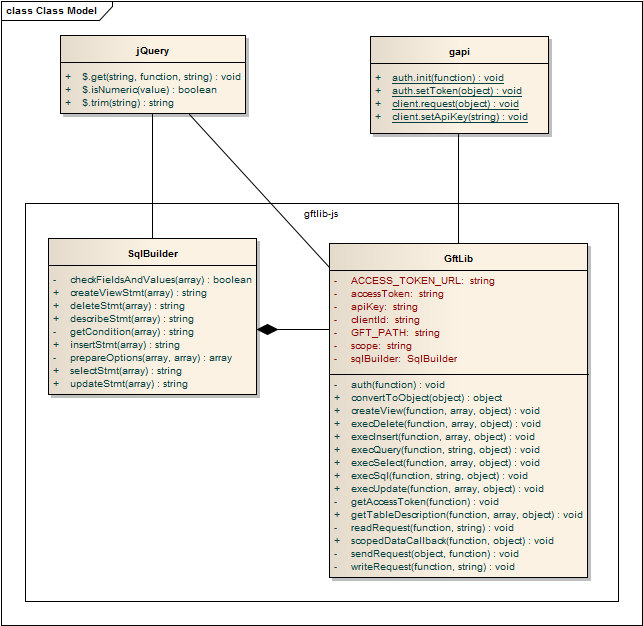
\includegraphics[width=0.8\textwidth]{images/gftlib-js/gftlibjs-classmodel}
	\caption{GftLib Klassendiagramm}
	\label{gftlibjs-classmodel}
\end{figure}

\subsection{Testing}
\label{gftlib-testing}
Mit Hilfe des Unit-Testing Frameworks QUnit\footnote{\url{http://docs.jquery.com/QUnit}} konnten wir für die GftLib durchgängige Tests erstellen. Die Tests wurden in JavaScript geschrieben und können deshalb direkt im Browser ausgeführt werden\footnote{Produktive Tests: \url{http://gft.rdmr.ch/test/js/}}. 

\begin{figure}[!ht]
	\centering
	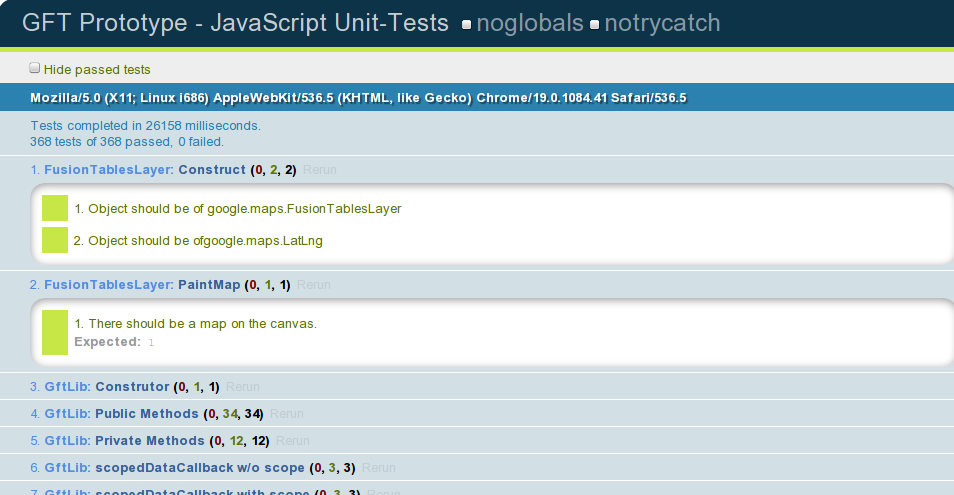
\includegraphics[width=0.8\textwidth]{images/gftlib-js/gftlibjs-tests}
	\caption{QUnit Tests der GftLib}
	\label{gftlibjs-tests}
\end{figure}

Wir haben insgesamt 84 Tests für die GftLib erstellt, welche jede Funktion mit verschiedenen Parametern prüft. Wir haben den \emph{test early}-Ansatz gewählt, dabei werden die Tests sehr zeitnah zur Erstellung einer Funktion geschrieben. Dank der guten Testabdeckung konnten wir unseren Code regelmässigen Refactorings unterziehen ohne uns darum Sorgen zu machen, bestehende Funktionalität kaputt zu machen (Regression). Es hat sich gezeigt, dass wir dadurch auch in der Lage waren, schnell auf das neue Trusted Tester \gls{API} (siehe Abschnitt \ref{trusted-tester-api}) zu wechseln, da wir nur sicherstellen mussten, dass unsere Tests wieder fehlerfrei durchlaufen. Dabei haben wir sogar einen Bug der Schnittstelle entdeckt, welchen wir Google gemeldet haben (siehe Abschnitt \ref{austausch-mit-google}).

QUnit hat sich als sehr wertvoll erwiesen bei den sogenannten asynchronen Tests. Obwohl unsere Bibliothek sehr stark auf die asynchronen Aufrufe des Google \gls{API}s angewiesen ist, konnten wir trotzdem normal Tests schreiben ohne uns speziell um diesen Aspekt kümmern zu müssen.

Wenn wir einen Bug gefunden haben, haben wir diesen jeweils mit einem Unit-Test nachvollzogen, so dass dieser nicht noch ein weiteres Mal auftritt. Die Testabdeckung haben wir mit JSCoverage\footnote{\url{http://siliconforks.com/jscoverage/}} gemessen, für die GftLib beträgt diese 95\%, beim SqlBuilder sogar 100\% (siehe Abbildung \ref{gftlibjs-testabdeckung}). Bei den fehlenden 5\% handelt es sich um die Fehlerbehandlung der asynchronen Aufrufe, welcher sich nicht so einfach testen lässt.

\begin{figure}[!ht]
	\centering
	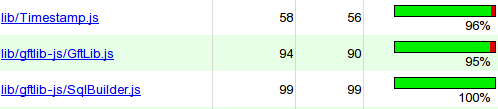
\includegraphics[width=0.5\textwidth]{images/gftlib-js/gftlibjs-testabdeckung}
	\caption{Gemessene Testabdeckung mit JSCoverage}
	\label{gftlibjs-testabdeckung}
\end{figure}

Private Methoden sind in JavaScript grundsätzlich nicht von aussen zugreifbar. Da sich ein Grossteil der Funktionalität in solchen privaten Methoden befindet, haben wir öffentliche Aliase erstellt, um Tests dieser Methoden zu ermöglichen. Die Aliase sind jeweils mit zwei Unterstrichen gekennzeichnet; sie sind nicht teil des öffentlichen \gls{API}s und sollten nur von von Unit-Tests verwendet werden.
